\chapter{FPGA usages in cryptography\label{FPGA_crypto}}
Due to the high demand on fast cryptographic methods, optimized implementations
became of huge interest. Hence the motivation behind developing faster FPGA
implementation of cryptographic schemes. In this chapter we are giving an
overview of optimized FPGA implementations for R-LWE.


The implementation as seen in Figure \ref{fig:high_level_pkc_impl} consist of
three different modules: key generation, encryption and decryption. These
modules consist of a few basic operations, polynomial multiplication,
polynomial addition, subtraction and scalar division to the nearest integer.
The most expensive complexity-wise is the modulo operation which can take a few
hundred LUTs. Which is why these designs try to minimize the amount of modulo
operations with operations such as conditional assignment
\citep{FPGA_Post_Quantum_Primitives}. The way the noise sampler and the true
random number generator works is out of the scope of this paper.

\begin{figure}[H]
    \centering
    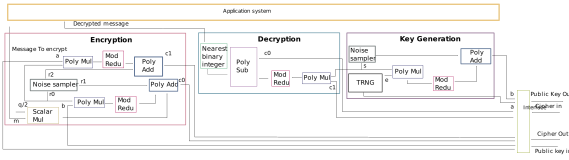
\includegraphics[scale=0.40, angle=90]{high_level_impl.png}
    \caption{An optimized high level implementation of the three building
    blocks for a public key cryptosystem \citep{FPGA_Post_Quantum_Primitives}}
    \label{fig:high_level_pkc_impl}

\end{figure}

\begin{itemize}

    \item
        In Figure \ref{fig:poly_add} and Figure \ref{fig:poly_sub} implement
        polynomial addition and subtraction respectively. They are the most
        common operations in the R-LWE cryptosystem and thus need to be fast.
        We compute the operation component wise and to avoid using the modulo
        operation we use conditional assignment.

        \begin{figure}[H]
            \centering
            \begin{subfigure}[b]{0.4\textwidth}
                \centering
                \includegraphics[scale=0.5]{polynomial_addition.png}
                \caption{Polynomial addition
                \citep{FPGA_Post_Quantum_Primitives}}

                \label{fig:poly_add}
            \end{subfigure}
            ~
            \begin{subfigure}[b]{0.4\textwidth}
                \centering
                \includegraphics[scale=0.5]{polynomial_subtraction.png}
                \caption{Polynomial subtraction
                \citep{FPGA_Post_Quantum_Primitives}}
                \label{fig:poly_sub}
            \end{subfigure}
        \end{figure}

    \item
        In Figure \ref{fig:scalar_mul} we implement scalar multiplication using
        multiplexers to save LUTs. Because $m$ is an $n$-bit vector, when
        computing $t\cdot m$ we essentially choose $t$ or $0$.

        \begin{figure}[H]
            \centering
            \includegraphics[scale=0.5]{scalar_multiplication.png}
            \caption{Scalar multiplication \citep{FPGA_Post_Quantum_Primitives}}
            \label{fig:scalar_mul}
        \end{figure}

    \item
        In Figure \ref{fig:scalar_div} we implement scalar division, let
        $d = (c_0 - s \cdot c_1)$ and $t = \frac{t}{2}$. When we want to
        compute the nearest integer we can compute $|d - t| < \frac{t}{2}$.
        Since $|d - t|$ measures the distance between $d$ and $t$; if the
        distance between the two is larger than $t / 2$ it means that $d$ and
        $t$ are far from each other, this means that $\frac{d}{t}$ the nearest
        integer will be $0$. On the other hand if $|d - t|$ is smaller than $t
        / 2$ it means that the nearest integer will be $1$.


        \begin{figure}[H]
            \centering
            \includegraphics[scale=0.5]{scalar_division.png}
            \caption{Scalar division \citep{FPGA_Post_Quantum_Primitives}}
            \label{fig:scalar_div}
        \end{figure}


    \item
        Polynomial multiplication is by far the most complex of these modules.
        Multiplication can change the degree of the polynomial, which increases
        the complexity of the component. It uses \textit{Number Theoretic
        Transform} (NTT) which is a generalized version of the discrete Fourier
        transform over the ring $R_q = R / \langle q \rangle = \bZ_q [x] / (x^n
        + 1)$ to compute the polynomials. The NTT equation is the following:
        let $\omega$ be the $n$-th root of unity for the polynomial $x^n + 1$.
        NTT is defined as the following equation

        \[ X_i = \sum^{n-1}_{j=0} x_j \cdot \omega^{i\cdot j}. \]

        $\omega$ has to satisfy the following conditions, firstly
        $\omega^n = 1 \mod q$. Secondly the period of
        $\omega^i \ \forall i \in \{1, 2, 3, \ldots, n - 1\}$ has to be exactly
        $n$.

        After computing the NTT of the vectors, we compute component wise
        multiplication. Using the \textit{Inverse NTT} (INTT) we convert it
        back to the correct form.

        The INTT is defined as \[X_i =
            n^{-1} \sum^{n-1}_{j=0} x_j \omega^{-ij}.\]


        \begin{figure}[H]
            \centering
            \begin{subfigure}[b]{0.4\textwidth}
                \centering
                \includegraphics[scale=0.5]{polynomial_multiplication.png}
                \caption{Polynomial multiplication \citep{FPGA_Post_Quantum_Primitives}}
                \label{fig:poly_mul}
            \end{subfigure}
            ~
            \begin{subfigure}[b]{0.4\textwidth}
                \centering
                \includegraphics[scale=0.25]{number_theoretic_transform.png}
                \caption{Number theoretic transform
                \citep{FPGA_Post_Quantum_Primitives}}
                \label{fig:ntt}
            \end{subfigure}
        \end{figure}

\end{itemize}


The number that is generally considered safe to use for $q$ is $q = 12289$.
Although any $q > 10 000$ with each polynomial having $128 - 1024$ coefficients
gets you the security level of at least 112 bits as recommended by NIST
\citep{barker2006recommendation}. This cryptosystem was implemented on a
Zynq-7000 FPGA, we can see the LUTs needed for different sizes of $n$ in Table
\ref{tab:hardwarecost}.

\begin{table}[H]
    \centering
    \begin{tabular}{l|ll}
        \textit{n} & LUTs   & Registers \\ \hline
        128        & 66251  & 16805     \\
        256        & 11490  & 33138     \\
        512        & 227458 & 65643     \\
        1024       & 426402 & 130540
    \end{tabular}
    \caption{Hardware cost using only LUTs where $q = 12289$
    \citep{FPGA_Post_Quantum_Primitives}}
    \label{tab:hardwarecost}
\end{table}

